\documentclass[landscape,pdftex]{jomislides}

\slidesmag{5} % escala, qto maior maiores ser�o as letras/figras/etc.

%\centerslidesfalse

%\usepackage{algorithmic}
\usepackage{alltt}
\usepackage{booktabs}
%\usepackage{algorithm}

%
% Slides
% ======
%


\begin{document}

%\input{autorHeaders}

\title{Data Science, Machine Learning and \textbf{Big Data}} 
\author{Fabr�cio J. Barth}
\institution{Professor da Faculdade BandTec \\ Cient�sta de Dados da
  VAGAS Tecnologia}
\date{Agosto de 2013}

\SlideHeader{}
            {}
\SlideFooter{\theslidepartheading $\;$ --- $\;$ \theslideheading}
            {\theslide}

\vpagecolor[white]{white}


\subtitle{}

\maketitle

%\begin{PartSlide}{\textbf{Import�ncia do Tema}}
%\end{PartSlide}

\begin{Slide}{Problema}
\begin{figure}[htbp]
\centering 
\resizebox*{1\columnwidth}{0.8\textheight}
{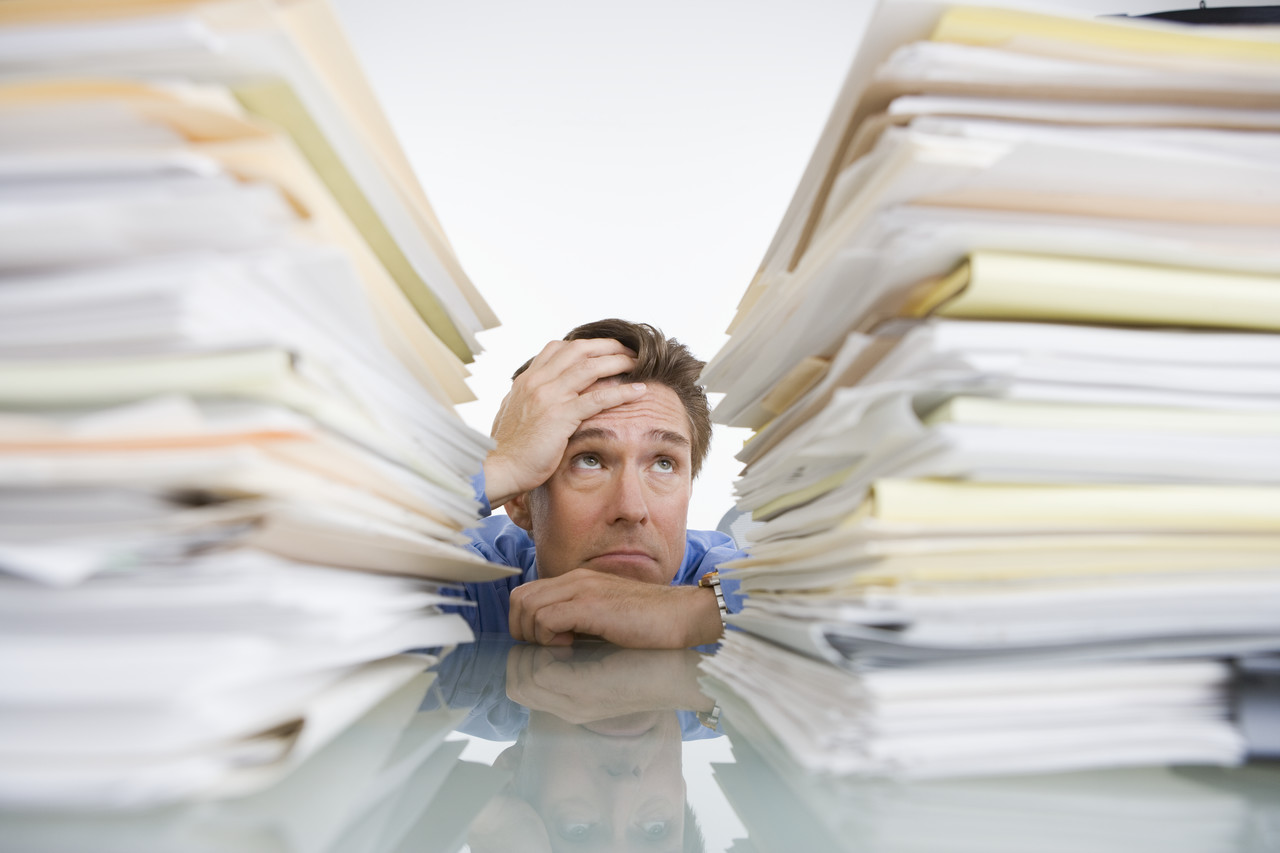
\includegraphics{figuras/information-overload.jpg}}
\end{figure}
\tiny
http://investingcaffeine.com/2010/01/07/tmi-the-age-of-information-overload/
\end{Slide}

\begin{Slide}{Alguns dados...}
\begin{figure}[htbp]
\centering 
\resizebox*{0.8\columnwidth}{0.8\textheight}
{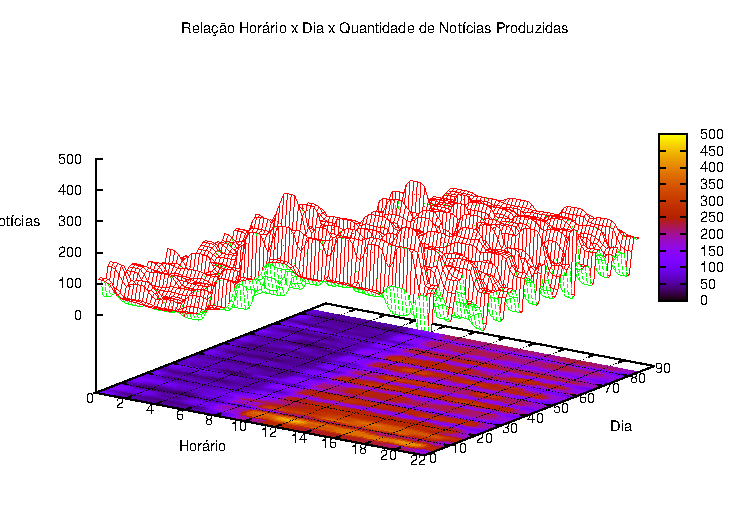
\includegraphics{figuras/notic_hor_dia_2.pdf}}
\end{figure}
\tiny
Quantidade de not�cias publicadas na Web por apenas seis
ve�culos brasileiros de not�cias ($D_{0}$ = 17/07/2007) 
\end{Slide}

\begin{Slide}{Dados mais atuais}
\begin{itemize}
\item A380: Heathrow $\rightarrow$ JFK: 640 TBs de log
\item Twitter: 12+ TBs of tweet every day
\item Facebook: 25+ TBs of log data every day
\item Sistemas baseados em RFID
\item Smartphones com GPS, aceler�metro, ...
\end{itemize}

\small
\textit{http://www.ibmbigdatahub.com/}\\
\textit{Mitchell. Mining our reality. Science. 2009}

\end{Slide}

\begin{Slide}{De onde vem os dados?}
\begin{figure}[htbp]
\centering 
\resizebox*{1\columnwidth}{0.6\textheight}
{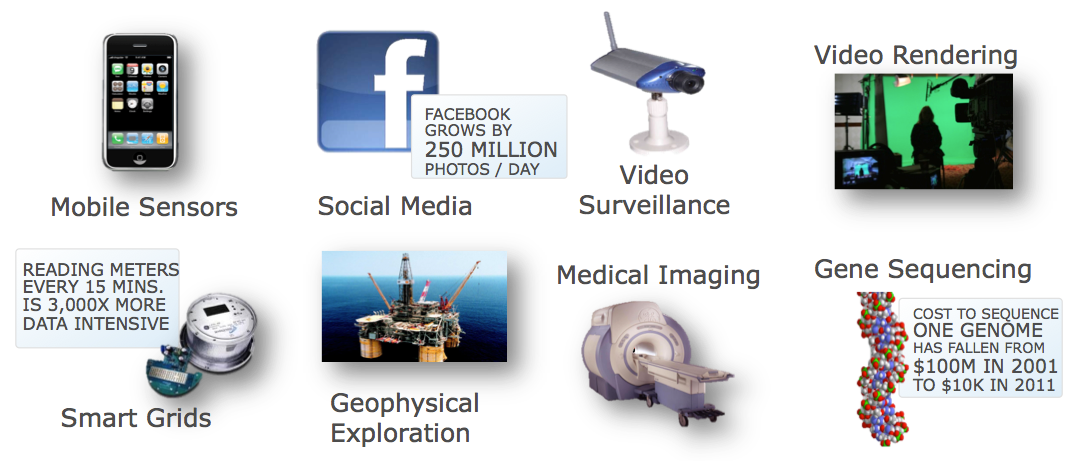
\includegraphics{figuras/data.png}}
\end{figure}
\tiny
Summer School on Big Data - EMC
\end{Slide}

\begin{Slide}{Mining our reality}
\begin{figure}[htbp]
\centering 
\resizebox*{0.8\columnwidth}{0.8\textheight}
{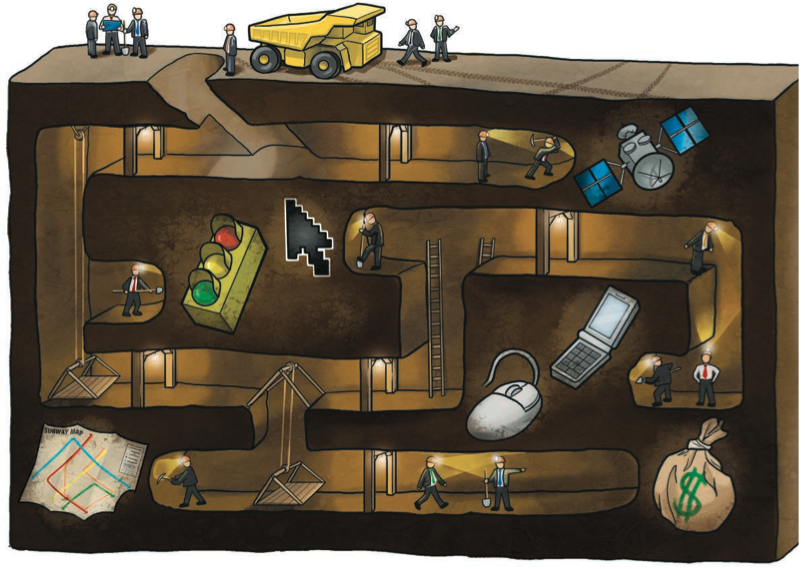
\includegraphics{figuras/mitchellScience.png}}
\end{figure}
\tiny
\textit{Mitchell. Mining our reality. Science. 2009}
\end{Slide}

%\begin{Slide}{Mais dados...}
%\begin{figure}[htbp]
%\centering 
%\resizebox*{0.8\columnwidth}{0.8\textheight}
%{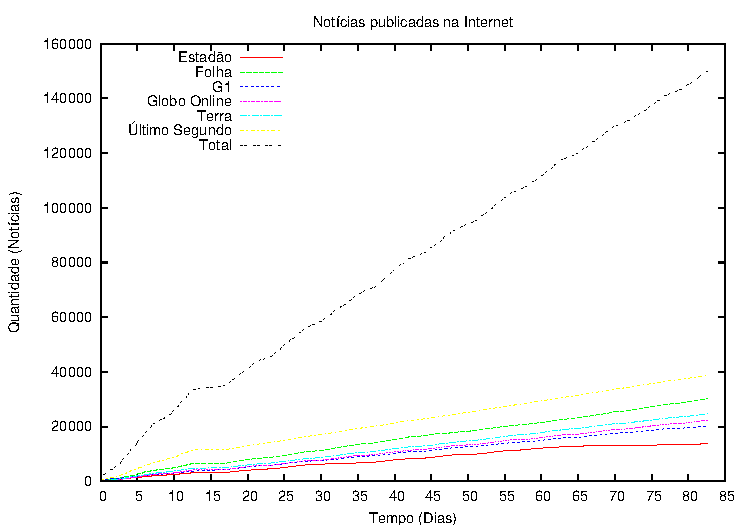
\includegraphics{figuras/noticias.pdf}}
%\end{figure}
%\tiny
%$D_{0}$ = 17/07/2007
%\end{Slide}


\begin{Slide}{Big Data}
\begin{figure}[htbp]
\centering 
\resizebox*{0.5\columnwidth}{0.7\textheight}
{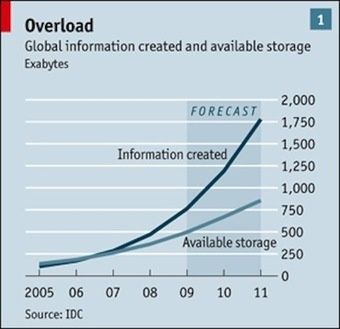
\includegraphics{figuras/bigData.jpg}}
\end{figure}
\tiny
\textit{``We collect an astonishing amount of digital information... ...we've
long since surpassed our ability to store and process it all. Big data
is here, and it's causing big problems...''}\cite{eco2010} 
\end{Slide}

\begin{Slide}{Big Data � um conceito relativo}
\begin{itemize}
\item O que � \emph{grande hoje}...
\item Pode n�o ser \emph{grande amanh�}...
\end{itemize}
\end{Slide}

\begin{Slide}{Big Data refers to...}
\begin{itemize}
\item All data that comes at high \emph{Volume}
\item All data that comes at high \emph{Velocity}
\item All data that comes from a \emph{Variety of Sources}
  (structured + unstructured data)
\end{itemize}
\end{Slide}

\begin{Slide}{Variety of sources}
\begin{figure}[htbp]
\centering 
\resizebox*{1\columnwidth}{0.6\textheight}
{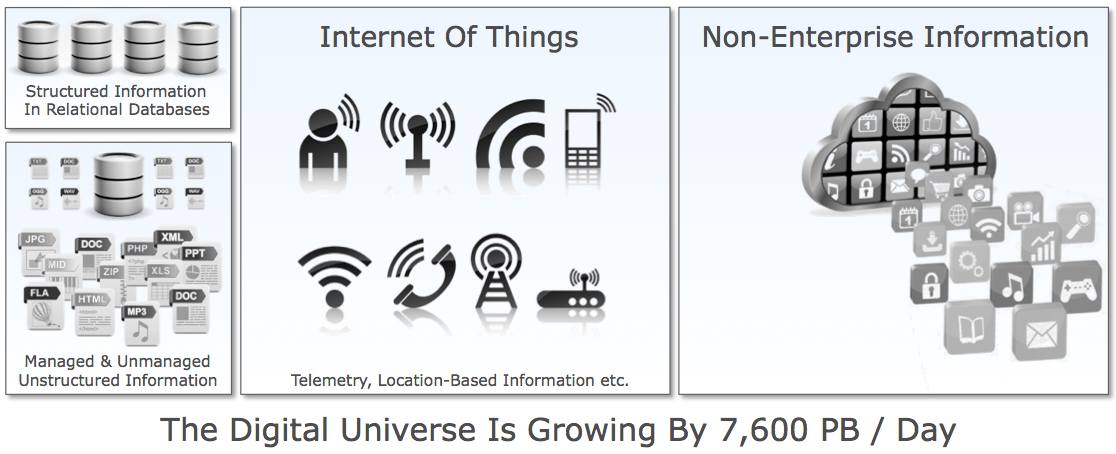
\includegraphics{figuras/data2.png}}
\end{figure}
\tiny
Summer School on Big Data - EMC
\end{Slide}

\begin{Slide}{Por que manipular este tipo de dado?}
\begin{itemize}
\item Identificar comportamento an�malo (i.e., fraudes, falhas) 
\item Sumarizar tend�ncias de publica��es de artigos e
  patentes sobre um determinado tema. 
\item Sumarizar e filtrar not�cias relevantes.
\newpage
\item Sumarizar a opini�o expressa na Web sobre a sua empresa.
\item Identificar padr�es de navega��o em sites.
\item Identificar conte�do impr�prio em sites.
\item Recomenda��o de livros, filmes, restaurantes e empregos.
\end{itemize}
\newpage

\end{Slide}

%\begin{Slide}{Exemplos de sucesso}
%\begin{itemize}
%\item Amazon
%\item Netflix
%\item xxx
%\end{itemize}
%\end{Slide}

\begin{Slide}{Data Scientist}
\begin{itemize}
\item \textit{Data Scientist: The Sexiest Job of the 21st Century. Harvard
  Business Review.}
\item \emph{Data Scientist} applies advanced \emph{analytical}
  tools and algorithms to generate \emph{predictive insights} and
  \emph{new} product \emph{innovations} that are a direct result
  of the data.
\end{itemize}
\end{Slide}

\begin{Slide}{Data Science Venn Diagram}
\begin{figure}[htbp]
\centering 
\resizebox*{0.6\columnwidth}{0.75\textheight}
{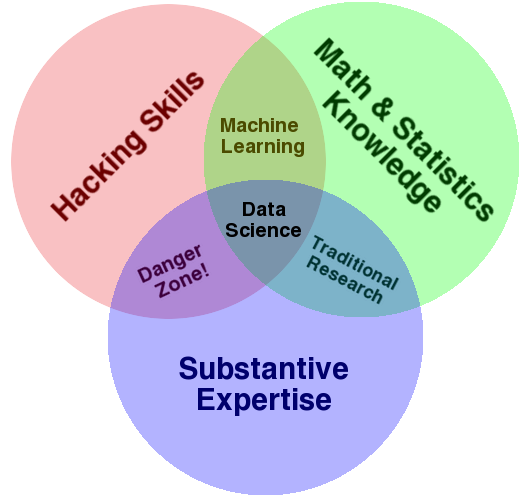
\includegraphics{figuras/Data_Science_VD.png}}
\end{figure}
\tiny
http://www.drewconway.com/zia/?p=2378
\end{Slide}

\begin{Slide}{Ciclo t�pico de um projeto}
\begin{figure}[htbp]
\centering 
\resizebox*{1\columnwidth}{0.8\textheight}
{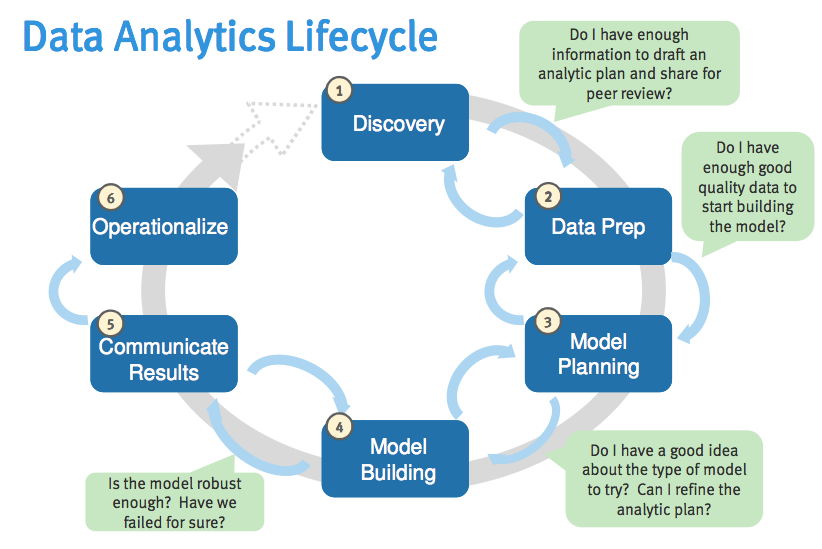
\includegraphics{figuras/ciclo.png}}
\end{figure}
\tiny
Summer School on Big Data
\end{Slide}


\bibliographystyle{plain}
\bibliography{doutorado,mestrado,publicacoes,atech,posDoutorado,vagas}

\end{document}

